%# -*- coding: utf-8-unix -*-

\chapter{结合共享账户的机票推荐算法}
\label{chap:share}

本章我们研究机票推荐中的共享账户问题,该问题主要针对一个用户ID包括多个乘客的情况。我们将提出一种算法,可以预测出用户下本次购票的乘客的概率分布,从而学习更具针对性的偏好模型,提升推荐准确率。

\section{机票推荐中的共享账户}

推荐算法总体分为两类,一类是根据用户和物品之间的关系,提出衡量用户相似度以及物品相似度的算法,为用户根据物品或用户之间的相似度提供推荐结果;另一类是基于内容的推荐,物品可以表示为特征的集合(包括显性特征和隐性特征),从用户的物品列表中学习用户对每个特征的偏好。为用户推荐最符合其特征偏好的物品。

以这两类算法为代表的传统推荐系统通常以用户在网站的注册ID(账户)来识别用户,它们一般假定一个用户背后只有一个使用者,即每个用户仅包含一个固定的偏好模型。然而在很多领域,都会发生现实中几个人共同使用一个账户的情景。例如,在购物网站,可能一个家庭共用一个账户,每位家庭成员都可以使用这个账户进行购物;在一般的线旅行票务服务网站,例如机票、酒店、旅游等业务领域,一个账户中也可能会有几个成员,他们可能会为家人、旅伴购票。


第一种情形中,虽然会有几位家庭成员共同使用账户购物,但是服务商无法获取购物者的真实身份信息。而对于第二种情形,如图\ref{fig:fill_id}所示,乘客在订票后会被要求填写身份信息,因此,网站可以获取其真实身份。在机票数据集中,订单包含了每一位乘客的身份信息,包括姓名、性别、年龄、证件号码等。在我们进行数据分析与实验过程中,统一使用加密后的证件号码来代指乘客,既确保了乘客之间无冲突,又保护了乘客隐私。

\begin{figure}
 \centering
 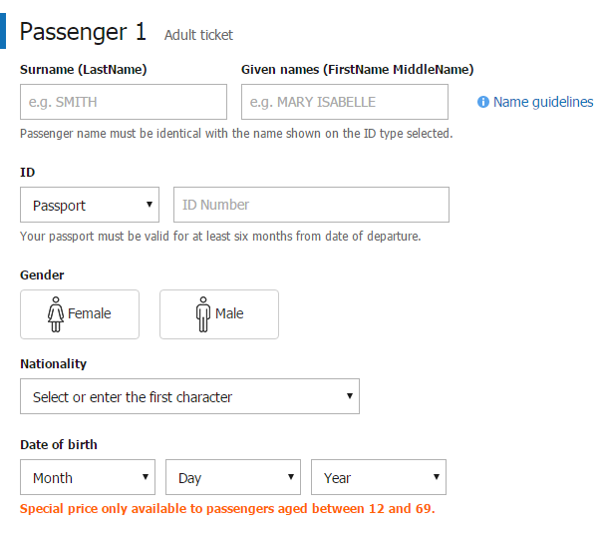
\includegraphics[width=0.7\linewidth,height=0.5\linewidth]{05/1_fill_id.png}
 \bicaption[fig:fill_id]{填写乘客信息}{用户在票务网站填写身份信息}{Fig}{Users Fill in Their Identification on Website}
\end{figure}

通常来说,同一个用户下乘客可能具有较为相似的偏好,但他们之间的差异也不能忽视。如果我们能够利用购票时获取的乘客身份信息为该乘客进行机票推荐,就可以为每位乘客建立特征分布模型,更具针对性的细粒度乘客模型对进一步提升个性化机票推荐准确率可以起到作用。然而,按照业务流程,只有当用户选定机票后才会填写身份信息。在我们进行机票推荐时还无法获取乘客信息。我们需要预测乘客的概率分布。

我们的问题是在共享账户的乘客选购机票时,根据乘客历史行为模式以及当前会话的上下文预测出本次购票的目标乘客。在电子购物网站等无法获得成员真实身份的场景中,为了解决共享账户问题,通常需要设置几个虚拟成员,其中每个成员代表一种偏好模型。虚拟成员的数量可以是固定值,也可以是通过模型计算出的最优值。然而,这类算法通常只分析用户和物品之间的关系,无法利用当前会话中的上下文信息;并且对虚拟成员预测的分布准确率也无法验证。在机票推荐场景中,对乘客的预测准确率是可以进行验证的。

在机票的乘客预测模型中,我们使用了作者主题模型(ATM)来分析乘客的行为模型。主题模型是一种生成模型,其主要观点是一篇文档可以抽取出混合的多个主题。作者主题模型在原主题的基础上又添加了作者的关系。每个账户独立进行模型训练,可以将每个账户看作一个语料库。账户中出现过的所有乘客看作每位作者,每条机票订单看作一篇文档, 机票中的每个特征以及上下文信息看作预定义的词库。如果出现一张机票有多个乘客的情况,我们将他们视为共同作者。

\section{乘客预测模型}
事实上,主题模型在推荐系统中的应用很广泛。例如,在PLSA模型中,每个物品可以视作一个词汇,主题服从对物品的多项式分布,每个主题代表了一种隐性特征。每用户的偏好模型都服从对主题的多项式分布。用户的每次购买行为都可以被看作从该用户中抽样一个主题$Z$,再从该主题中抽取一个词汇的过程。由于机票具有动态属性,很难将不同价格的机票定义为同一个物品;并且每类机票的数量受限于飞机的型号,因此上述pLSA模型很难用到机票推荐领域中。

\subsection{模型描述及表示}

在作者主题模型中,我们用机票在每个特征离散化后的取值来预定义一个词库。这个词库包含了机票在任一特征中所有可能出现的值,使用从0开始的索引来代指每一个词汇。至此,每一张机票都可以表示为词汇的集合,我们将每条订单视作一篇文档,显然,所有订单文档中的的词汇数量都是相同的。每个主题都由词汇的多项式分布表示;类似地,每个乘客由主题的多项式分布表示。因此
ATM模型可以对文档(订单)进行降维。通过模型训练,可以计算出乘客与主题之间的分布参数以及主题与词汇之间的分布参数。表\ref{tab:notation}描述了我们本章使用的符号表。

\begin{table}[!hpb]
\centering
  \bicaption[tab:notation]{符号表}{乘客预测模型符号表}{Table}{Notation for ATM}
\begin{tabular}{|c|c|} \hline
$M$ & 数据集账户数量\\ \hline
$V$ & 词库中单词的数量\\ \hline
$O$ & 一个账户中所有订单\\ \hline
$P$ & 一个账户中所有乘客\\ \hline
$P_i$ & 订单$O_i$对应的乘客集合 \\ \hline
$F$ & 机票特征集合\\ \hline
$K$ & 主题数量\\ \hline
\end{tabular}
\end{table}

对于一个账户$M$,我们获取其中包含的乘客集合$P$。我们使用矩阵$\Theta$来表示每位乘客的主题分布,这个参数矩阵的维度是$|P| \times K$,$K$代表模型主题的数量。$\Theta$以狄利克雷分布作为先验,该先验的超参数是$\alpha$。矩阵$\Phi$可以表示每个主题在词汇上的分布,该矩阵的维度是$V \times K$。$\Phi$同样以超参数为超参数是$\beta$的狄利克雷分布作为先验。通常情况下,超参数不是通过训练得到的,而是根据多次数据实验的经验总结来赋值。本章中,我们将$\alpha$赋值为$50/K$,将$\beta$赋值为0.01。

式\ref{eq:dir}描述了狄利克雷分布。其中,带$\Gamma$函数的那一项是常系数。可以发现,狄利克雷分布与多项式分布具有相同的形式。这两个分布是共轭分布。

\begin{eqnarray}
\label{eq:dir}
	Dir(\mathbf{p}|\alpha) & = & \frac{1}{B(\alpha)}\prod_{i=1}^n p_i^{\alpha_i-1} \nonumber \\
	& = & \frac{\Gamma(\sum_{i=1}^n \alpha_i)}{\prod_{i=1}^n \Gamma(\alpha_i)}\prod_{i=1}^n p_i^{\alpha_i-1}
\end{eqnarray}

在训练数据中,一条机票订单的乘客集合是明确的,每张机票的特征内容,即该文档的所有词汇也是明确的;为了训练两个矩阵参数,我们需要为订单中的每个词汇赋予乘客与主题。这两个变量属于隐性变量。首先我们从这条订单的乘客列表中按均匀分布抽取出一位乘客;然后根据乘客-主题参数矩阵抽取出一个主题$Z$,再根据主题-词汇参数矩阵抽取一个单词$w$,我们使用下列流程对生成模型进行数学描述:

\begin{enumerate}
\item 对每个账户中的所有乘客$p$,以狄利克雷先验初始化 $\Theta_p \sim Dir(\alpha)$
\item 对每个主题$t$,以狄利克雷先验初始化 $\Phi_t \sim Dirichlet(\beta)$
\item 对账户下的每条订单$o$
       \begin{enumerate}[fullwidth,itemindent=1em,label=(\alph*)]
       \item $P$ 表示这条订单的乘客集合
       \item 对于订单中的每一个词汇
              \begin{enumerate}[fullwidth,itemindent=2em,label=(\roman*)]
              \item 按均匀分布从$P$中抽取一位乘客 $X_{oi} \sim Uniform(P)$
              \item 从乘客-主题矩阵中抽取一个主题 $Z_{oi} \sim Multi(\theta_{X_{oi}})$
              \item 从主题-词汇矩阵中抽取一个单词 $w_{oi} \sim Multi(\phi_{Z_{oi}})$
              \end{enumerate}
       \end{enumerate}
\end{enumerate}

图\ref{fig:pro_graph}展示了作者主题模型的概率图。带阴影的变量是已知变量;其余是未知变量。每个方框代表一个过程,其右下角的数字是这个过程的循环次数。箭头连接线代表了变量间的条件依赖关系。这个图直观、清晰地表现了生成一条订单文档的过程。

\begin{figure}
 \centering
 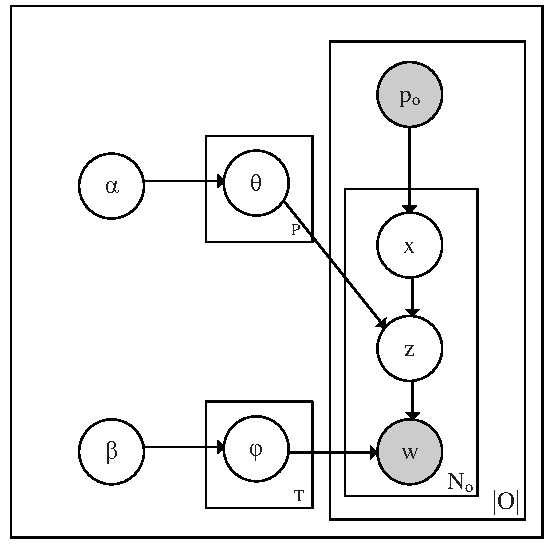
\includegraphics[width=0.45\linewidth]{05/2_graph.pdf}
 \bicaption[fig:pro_graph]{模型概率图}{作者主题模型的概率图}{Fig}{Probability Graph for the Author-topic Model}
\end{figure}

\subsection{模型参数推导}
在上节的模型描述中,我们介绍了作者主题模型的两个参数矩阵,分别是包含$P$位乘客的乘客-主题分布参数以及包含$K$个主题的主题-词汇分布。有一些算法可以用来推导这些参数,如EM算法、Gibbs采样等。传统的EM算法可能会陷入局部最优问题,并且这种算法的计算复杂性较高。本章,我们使用Gibbs采样的算法,这种算法不直接进行参数推导,而通过计算抽取的乘客和主题的后验分布,对参数进行更新。因此计算过程较为简单。


\begin{eqnarray}
\label{eq:all_pro}
P(\mathbf{w}_o | \Theta,\Phi,P) & = & \prod_{i=1}^{N_o}P(w_{oi}|\Theta,\Phi,\mathbf{p}_o) 
\nonumber \\
 & = & \prod_{i=1}^{N_o}\sum_{p=1}^{|P|}\sum_{t=1}^{K}P(w_{oi}|z_{oi}=t,\Phi)
P(z_{oi}=t|x_{oi}=p,\Theta)P(x_{oi}=p|\mathbf{p}_o) \nonumber \\
 & = & \prod_{i=1}^{N_o}\frac{1}{|P|}\sum_{p \in p_o}\sum_{t=1}^{K}\phi_{w_{oi}t}\theta_{tp}
\end{eqnarray}


式\ref{eq:all_pro}描述了在参数矩阵$\Theta$,$\Phi$和乘客集合$P$的条件下,生成一条机票订单的概率函数。在这个生成模型中,$P(w_{oi}|z_{oi}=t,\Phi)$是在选定主题的条件下,根据主题-词汇分布矩阵抽取单词的概率。
$P(z_{oi}=t|x_{oi}=p,\Theta)$是在选定乘客的条件下,根据乘客-主题分布矩阵抽取主题的概率。$P(x_{oi}=p|\mathbf{p}_o)$是乘客集合中以服从均匀分布抽取乘客的概率。这个等式可以看作生成一条订单的似然函数。如果将参数$\Theta$,$\Phi$视为随机变量,我们训练模型的目标就是训练变量,使概率函数具有最大后验分布(MAP, Maximum A Posteriori)。 

在Gibbs采样的过程中,为了从联合分布$P(\mathbf{z},\mathbf{x}|\alpha,\beta)$中取样,我们需要为每一个单词$w_{di}$赋值一个主题$z_{di}$以及乘客$x_{di}$。在训练过程中,一个账户下的所有单词都会被取样一次。当所有单词都训练过,称为一个训练批次。通常,我们需要将模型训练数个批次。$p(\Theta,\Phi|\mathbf{z},\mathbf{x},\alpha,\beta)$可以根据狄利克雷和多项式分布四共轭分布的性质来计算。为每个单词抽取的乘客、主题可以使用下式进行计算:

\begin{eqnarray}
\label{eq:pro_pass_top}
P(x_{oi}=p,z_{oi}=t|w_{oi}=w,\mathbf{z}_{-oi},\mathbf{x}_{-oi},\mathbf{w}_{-oi},\alpha,\beta,p_o) \nonumber\\
\propto \frac{C_{tp}^{TP}+\alpha}{\sum{t'}C_{t'p}^{TP}+T\alpha}\frac{C_{wt}^{WT}+\beta}{\sum_{w'}C_{w't}^{WT}+W\beta}
\end{eqnarray}

式\ref{eq:pro_pass_top}代表为订单$o$的第i个单词赋予乘客p和主题t的概率。$C^{WT}$ 是单词-主题分布矩阵,其每行对应一个单词,每列对应一个主题,每个值代表当前单词被赋予当前主题的次数。$C_{wt}$是除了当前单词之外,单词$w$被赋予主题$t$的次数。$C^{TP}$是主题-乘客分布矩阵,其每行对应一个主题,每列对应一个乘客,矩阵中每个值代表对与该乘客在当前主题包含的单词个数。$C_{tp}$代表乘客$p$在主题$t$包含的词汇个数,同样排除了当前单词。我们可以根据抽样的过程对主题-词汇分布参数以及乘客-主题分布参数进行更新:

\begin{equation}
\label{eq:es_the}
\theta_{tp} = \frac{C_{tp}^{TP}+\alpha}{\sum{t'}C_{t'p}^{TP}+T\alpha}
\end{equation}

\begin{equation}
\label{eq:es_phi}
\phi_{wt} = \frac{C_{wt}^{WT}+\beta}{\sum_{w'}C_{w't}^{WT}+W\beta}
\end{equation}

式\ref{eq:es_the}和式\ref{eq:es_phi}分别两个参数的更新公式。$\theta_{tp}$是主题t在乘客p上的概率分布;$\phi_{wt}$是单词w在主题t上的概率分布。在每次取样后,
需要为每条订单更新单词-主题列表$T$以及单词-乘客$P$列表,其中$T[o][i]$代表在订单$o$中第$i$个单词的主题;$P[o][i]$代表在订单$o$中第$i$个单词的作者。因此,在参数推导的过程中,
我们需存储上文提到的$C^{TP}$和$C^{WT}$两个矩阵,以及每条订单中每个单词的主题和乘客两个列表。


模型训练主要包括三个步骤,分别是初始化,取样以及参数更新。在初始化过程中,我们为语料库中每条订单文档的每个单词随机分配主题和乘客。然后我们需要统计词汇表中每个单词被赋予某个主题的次数以及每个乘客在每个主题下的词汇的个数。在每次取样过程中,我们根据式\label{eq:p_xz}为语料库中的每个单词计算每个主题以及乘客的联合概率分布。我们根据概率为该单词采样新的主题和乘客。在几个批次的迭代训练后,可以根据式式\ref{eq:es_the}和\ref{eq:es_phi}对参数矩阵$\Theta$,$\Phi$进行更新。

在最差情况下,模型每批迭代的时间复杂度是$O(NK|P|)$。其中$N$是一个账户下所有订单的总词汇数量。$|P|$是该账户下乘客最多的订单中乘客的数量,一般不会很大,与订单的总词汇数量相比可以视作常量。$K$是模型的主题数量。主题数量的取值不是固定的,我们可以在实验中确定最适合机票推荐业务中,乘客预测模型的数量。在模型迭代过程中,$|P|$以及$K$都可以看作常量,因此,使用Gibbs采样训练ATM模型的时间复杂度可以看作与总订单词汇数量$N$呈线性关系,可以用在大量用户数据的训练任务中。

\begin{algorithm}
\caption{ATM模型训练}
\label{algo:atm_train}
\begin{algorithmic}[1]
\Require
\Statex 账户历史订单转化词汇表 $W$

\Ensure 
\Statex 乘客-主题分布参数 $\Theta$
\Statex 主题-词汇分布参数 $\Phi$

\State $nak , nkv, nak\_sum, nkv\_sum \gets 0$
\State $pl , tl \gets 0$
\For{$o \in W$}
\For{$w \in o$}
\State Pick a topic $t$ and a passenger $p$ uniformly;
\State passenger-topic count $nak[p][t] += 1$;
\State passenger-topic sum $nak\_sum[p] += 1$;
\State topic-word count $nkv[t][w] += 1$;
\State topic-word sum $nkv\_sum[t] += 1$;
\State word-topic list $tl[o][w] = t$
\State word-passenger list $pl[o][w] = p$
\EndFor
\EndFor
\While {not reach iteration limit}
\For{$o \in W$}
\For{$w \in o$}
\State $nak[p][t] -= 1, nak\_sum[p] -= 1$;
\State $nkv[t][w] -= 1, nkv\_sum[t] -= 1$;
\State Sample a new passenger $p'$ and topic $t'$ by Eq \ref{eq:pro_pass_top};
\State $nak[p'][t'] += 1, nak\_sum[p'] += 1$;
\State $nkv[t'][w] += 1, nkv\_sum[t'] += 1$;
\State $tl[o][w] = t', pl[o][w] = p'$;
\EndFor
\EndFor
\EndWhile
\State Calculate $\Theta,\Phi$ by Eq \ref{eq:es_the},\ref{eq:es_phi};
\State \Return $\Theta,\Phi$;
\end{algorithmic} 
\end{algorithm}

算法\ref{algo:atm_train}描述了ATM模型的训练过程。该过程的输入是账户下历史订单根据预定义词库转化的词汇表;输出是两个参数矩阵。其中第1至13行是模型初始化过程;其中第14至25行是使用Gibbs取样过程,每次取样将单词的乘客和主题进行更新,在计算过程中,我们增加了两个矩阵存储中间变量的结果;最后两行对参数进行更新。

\subsection{使用ATM模型进行乘客预测}

上一节我们介绍了在机票推荐领域中作者-主题模型的训练过程。我们首先定义一个词库,将账户下所有订单用作训练,并最终得到参数矩阵$\Theta$和$\Phi$。我们的目的是利用ATM模型,预测当前会话中账户下所有乘客购票概率分布。该问题在本质上属于分类问题,我们可以计算出每位乘客的购票概率,按概率将乘客进行排序。排位越靠前的乘客,越可能是本次购票者。

\begin{equation}
\label{eq:pred_pass}
p(x=p|o_n,\Theta,\Phi) \propto p(p)\prod_{w \in o_n}\sum_t p(t|w)p(w|t,p)
\end{equation}

式\ref{eq:pred_pass}的含义是在参数$\Theta$,$\Phi$的条件下,词汇集合$o_n$属于乘客$p$的的概率,相当于$p$属于订单$o$的乘客的概率。第一项的含义$p(p) = |O_p| / |O|$,$|O_p|$是训练集中乘客$p$参与的订单数量;$p(w|t,p)$是在给定主题和乘客的条件下,取样单词$w$的概率,由于从乘客中采样主题与从主题中采样单词的过程相互独立,因此$p(w|t,p) = p(t|p) \times p(w|t)$。$p(t|w)$代表单词$w$被赋予主题$t$的概率,可以通过迭代完成后的$C^{WT}$矩阵计算出来。

在乘客预测过程中的还有一个问题需要注意。我们在训练模型时可以使用订单的全部特征内容作为词汇列表;然而在机票推荐场景下,我们无法获得用户将要选购的机票的所有特征内容,因此不能用与训练数据一样的词汇表。因此,我们需要挖掘更多可能获取的特征,如起飞城市、到达城市、订票提前天数、登录网站的时间、IP地理位置等信息;以及用户行为上下文,包括搜索、点击、筛选等行为。因此我们在训练模型时,除了收集机票的特征,还需要将这些信息也转化为词汇,一并参与训练。

获取了每位乘客的概率分布后,为了针对乘客进行建立更细粒度的偏好模型,我们需要提供确切的参与该订票会话的乘客列表。平均每位乘客的概率是$\frac{1}{|P|}$,而我们只取概率超过平均概率的乘客。将这部分乘客视作参与本次订票的乘客集合。

至此,我们使用作者-主题模型对当前会话的乘客进行了预测,预测过程总体分为两个步骤。第一步,我们生成了一个预定义词库,使用Gibbs采样迭代训练了模型参数矩阵$\Theta$和$\Phi$;第二步,我们使用公式\ref{eq:pred_pass}为当前会话的乘客概率分布进行预测,并最终决定了参与本次订单的乘客集合。

\section{结合乘客预测的机票个性化推荐}
上一节介绍了机票推荐中的乘客预测算法,本节我们将乘客预测结合到个性化机票推荐中。旨在细化偏好模型的粒度,为乘客建立更有针对性的特征分布模型。进一步提升推荐准确率。

\begin{figure}
 \centering
 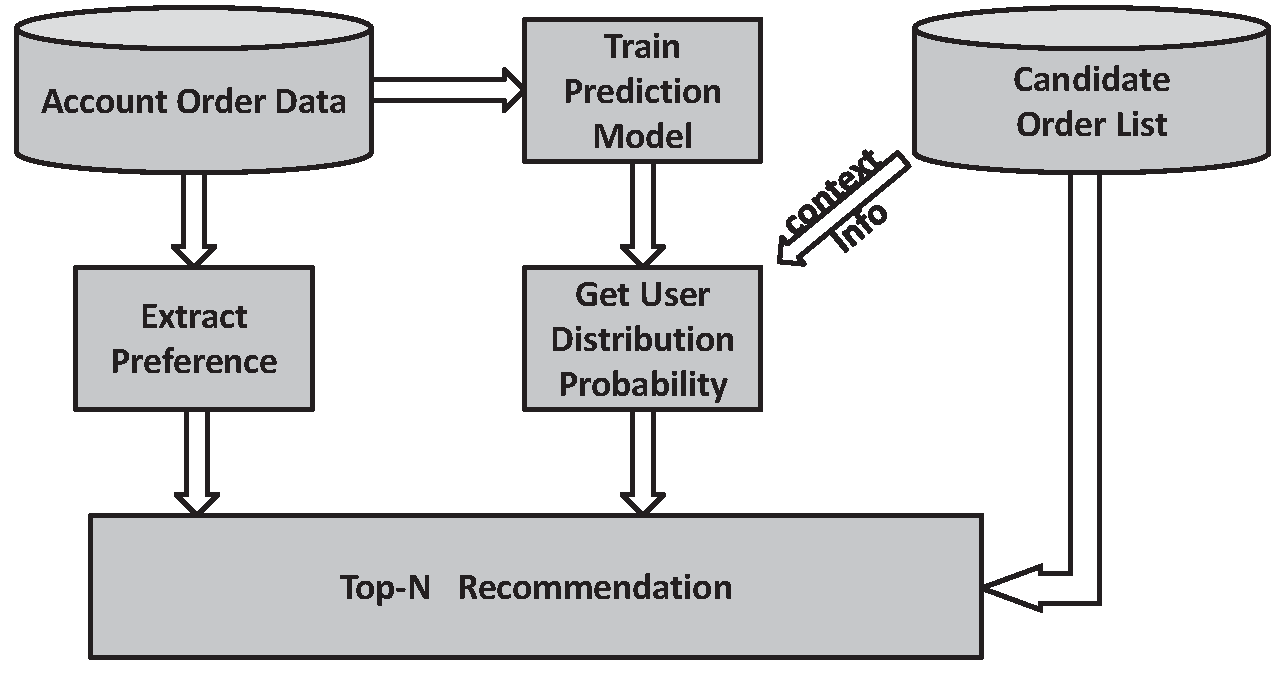
\includegraphics[width=0.6\linewidth]{05/3_overview.pdf}
 \bicaption[fig:over_pr]{预测推荐概览}{结合乘客预测的机票推荐概览}{Fig}{Overview of Passenger Prediction based Recommendation}
\end{figure}

图\ref{fig:over_pr}是结合乘客预测的机票推荐流程概览图。我们的数据源是存储在数据仓库中的用户机票订单数据。一方面我们可以利用这部分数据进行作者-主题模型训练,将训练后的模型用于乘客预测;另一方面,这部分数据还用来构建表示用户偏好的特征分布模型,这里我们不根据账户ID为粒度进行建模,而是为账户中每一位乘机人建立模型。这两个部分都是可以进行离线计算的。此外我们还结合在用户购票会话中的上下文信息,进行乘客预测;并结合乘客预测和机票推荐的结果,对候选机票列表进行排序,得到最终推荐结果。

然而,每位用户的乘客预测模型并不是一成不变的。用户每购买一次机票,我们都需要为该账户更新ATM模型,将本次订单包括进去。最佳的更新策略是每添加一条新的订单时,都重新训练模型,但这会带来计算效率低下的问题。我们可以使用一种蒙特卡洛算法进行更新,这种更新策略只关注新订单中的词汇,因此我们可以快速为新订单中的词汇赋值乘客与主题。首先,我们将该条订单中的词汇随机赋予乘客与主题;然后我们对新订单中的词汇按照式\ref{eq:pro_pass_top}重新取样乘客和主题,并更新矩阵$C^{TP}$和$C^{WT}$,最终更新两个参数矩阵。由于新订单中词汇较少,只需要十次左右的迭代过程就可以完成训练。

获取到乘客的概率分布并选取出参与当前订单的乘客后,我们将这些乘客的特征分布模型读取出来,并进行融合。融合的策略可以按照计算出的乘客分布概率进行加权,我们除了考虑乘客分布概率外,还需要考虑乘客的订单总量,这里我们给出乘客特征分布模型的融合策略:
\begin{equation}
	\label{eq:dis_com}
	\mathbf{D'} = \sum_{p \in P'} p(x = p|o_n,\Theta,\Phi) * \log |O_p| * \mathbf{D_p}
\end{equation}

式\ref{eq:dis_com}给出了多乘客的特征分布融合公式。其中$P'$是本次会话预测的参与乘客集合。我们为每位乘客赋予的权重是该乘客的参与概率以及该乘客参与的订单数量取以10为底的对数。得到了融合的特征分布模型后,我们就可以将之用在机票推荐上。

\section{实验结果分析}

本节我们对前几节提出的基于作者-主题模型的乘客预测及机票推荐算法进行实验评估与分析。

\subsection{实验数据集与评价指标}

\subsubsection{实验数据集描述}
我们的实验数据集是用户在多航线上的机票订单数据。数据以用户ID区分每个账户,以订单ID区分每条订单,以加密后的乘客证件号区分订单中的每位乘客。数据集引入乘客字段后,每个订单ID可能对应多条订单数据副本,每个副本之间唯一的差别就是乘客ID字段。我们取乘客数量在2至5人的网站账户,如果乘客数量过多,这个账户可能是代理账户,并且每位乘客订单比重很小。不适合用于训练乘客预测模型。

除了从数据仓库中直接拉取的账户训练数据外,我们还生成了一份虚拟账户数据。在一些共享账户推荐问题的研究中会用到虚拟账户数据。一般的做法是将两个或多个账户的数据合并为一个账户。由于账户的偏好模型具有较为明显的差异,在研究中可以将每个真实账户的模型视作虚拟账户中的一个成员。使用这类数据可以充分挖掘共享账户中的特征差异。另外,一般的共享账户问题缺少准确的账户成员信息,无法验证实验结果,而使用虚拟账户数据同时可以作评价实验结果的依据。

在我们的问题中,每位乘客的身份信息是明确的,我们生成虚拟账户数据的目的是探究乘客间的偏好差异对乘客预测以及机票推荐准确率的影响。我们的生成策略是在随机的两个账户中取一位乘客,并将这两位乘客合成一个乘客。如果两位乘客有同一个航班在同一起飞日期的订单,我们随机删除一条订单。

\subsubsection{乘客预测与机票推荐的评价指标}

对于一条订单数据,乘客预测的评价指标是预测正确的乘客数量,我们使用下式来评价乘客预测的准确率:
\begin{equation}
\label{eq:pass_acc}
Acc(o_i) = \frac{P' \cap A}{\sqrt{|P'| \times |A|}}
\end{equation}

式\ref{eq:pass_acc}中,$|P'|$是我们预测的乘客列表,$A$是本条订单实际乘客列表,对每条测试数据而言是一个固定值。其中分子项是预测乘客与实际乘客的交集;分母项是预测乘客与实际乘客各自数量的乘积,是一项惩罚项。可以看出,如果预测乘客与实际乘客集合完全相等,则准确率是1;如果预测乘客没有命中任何一位实际乘客,则准确率是0;在预测准确的乘客数量固定的前提下,预测乘客越多,准确率越低。

对于机票推荐,我们使用式\ref{eq:a-rec}对每条机票推荐准确率进行评价,
以及式\ref{eq:ma}对每种模型下所有用户的推荐平均准确率进行评价。除此之外,考虑到实际应用场景。
我们还增加了$Top-N$评价指标:

\begin{equation}
\label{eq:topn}
top-N = \frac{\sum_{i=1}^{|M|}|top-N(u_i) \cap O_{u_i}|}{|M|}
\end{equation}

对一次推荐而言,如果推荐列表中前$N$条候选机票包含了用户实际选择的机票,则认为推荐成功,否则就认为推荐失败。$Top-N$准确率是对所有推荐的平均准确率。可以直观衡量推荐的效果。


\subsection{乘客预测准确率}
本小节我们对乘客预测的准确率进行评价。我们为每个账户训练作者-主题模型,并在测试订单上进行乘客预测。
\begin{figure}
\centering
\subfigure[真实账户乘客预测准确率]{
 \label{fig:pre_acc_r}
 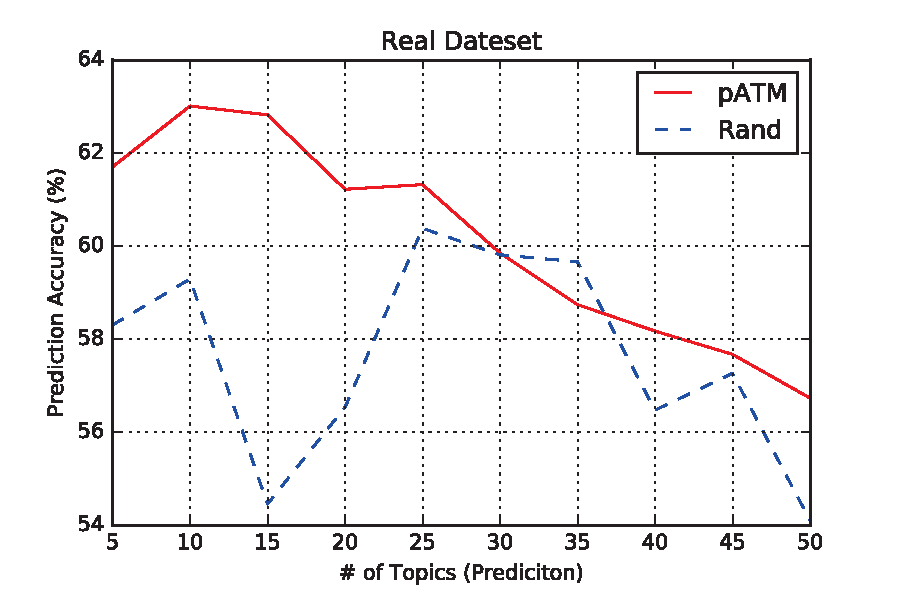
\includegraphics[width=0.49\linewidth]{05/4_pred_real.pdf}}
\subfigure[虚拟账户乘客预测准确率]{
 \label{fig:pre_acc_a}
 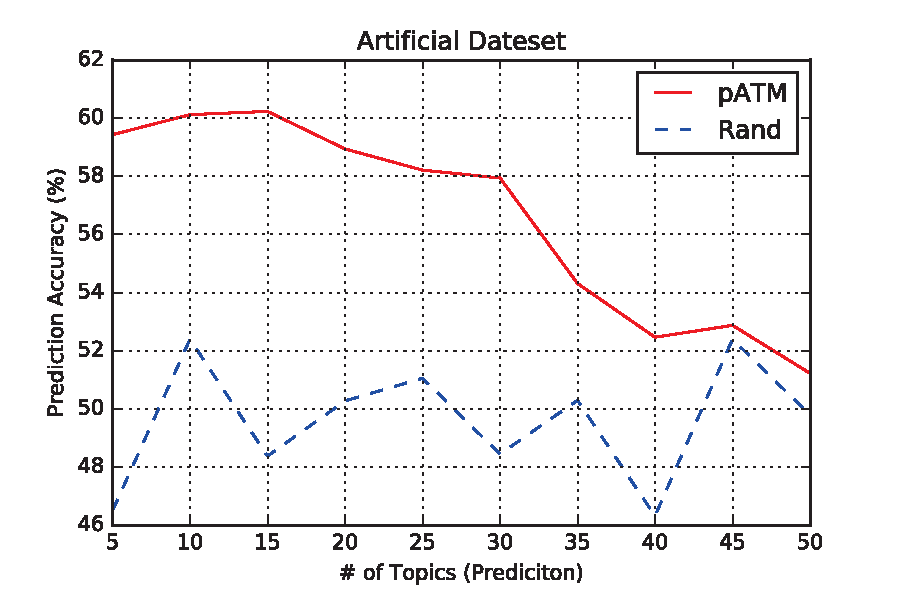
\includegraphics[width=0.49\linewidth]{05/5_pred_arti.pdf}}
\bicaption[fig:pred_acc]{乘客预测}{两个数据集上乘客预测准确率}{Fig}{Mean Accuracy for Passenger Prediction on Datasets}
\end{figure}

图\ref{fig:pred_acc}展示了乘客预测的实验结果。其中图\ref{fig:pre_acc_r}是在真实账户数据集的实验结果;图\ref{fig:pre_acc_a}是在虚拟账户数据集的实验结果。
其中,横轴是主题数量,范围从5到50共10个取值。进行乘客预测的两种方法分别是作者-主题模型(pATM)预测以及随机预测(Rand)。在随机预测中,我们同样取10个随机值。

可以看到,在真实账户数据集中,随机乘客预测的平均准确率在$57\%$左右,而ATM模型的最高预测准确率是$63\%$。在虚拟账户数据集中,随机乘客预测的平均准确率在$50\%$,因为每个虚拟账户只有两位乘客,而我们每次仅选取一位乘客;并且每条订单的乘客数量也是1。而ATM模型的最高预测准确率是$60\%$。可以看到,在真实数据集中的乘客预测准确率略高与虚拟数据集。
其原因是预测准确率同时和预测乘客以及实际乘客的数量有关,在不同的数据集上有不同的基准值。而随机算法在一定程度上可以反映出这个基准值。因此我们的主要标准是衡量ATM模型准确率对随机预测算法的提升。

可以看到,在虚拟账户上准确率的提升高于真实帐户。因为虚拟账户的乘客间差异更大,更有利于提取各自的特征。在真实账户数据集,乘客预测的准确率对比与随机预测有所提升。在两个数据集上,预测准确率都与主题的数量相关。当主题数少于15时,预测准确率保持在较高的水平;而随着主题数的增加,准确率有所下降;通过观察训练参数我们发现,过多的主题数会增加参数矩阵的稀疏性,进而影响到预测准确率。在两个数据集上,预测准确率都是在主题数为10的情况下达到最高值,这证明了ATM模型对同构的文档具有较稳定的表现。
在下一小节机票推荐部分中,我们将乘客预测模型的主题数量固定为10。


\subsection{机票推荐准确率}
本小节我们为账户(用户)进行机票推荐,虽然已经训练了乘客预测模型,并且进行了乘客粒度的特征分布模型学习。在实际应用中,机票推荐还是在用户粒度进行的。我们将从基于排序的推荐准确率和$Top-N$准确率两个角度进行衡量。

\begin{figure}
\centering
\subfigure[真实账户推荐准确率]{
 \label{fig:pre_rec_r}
 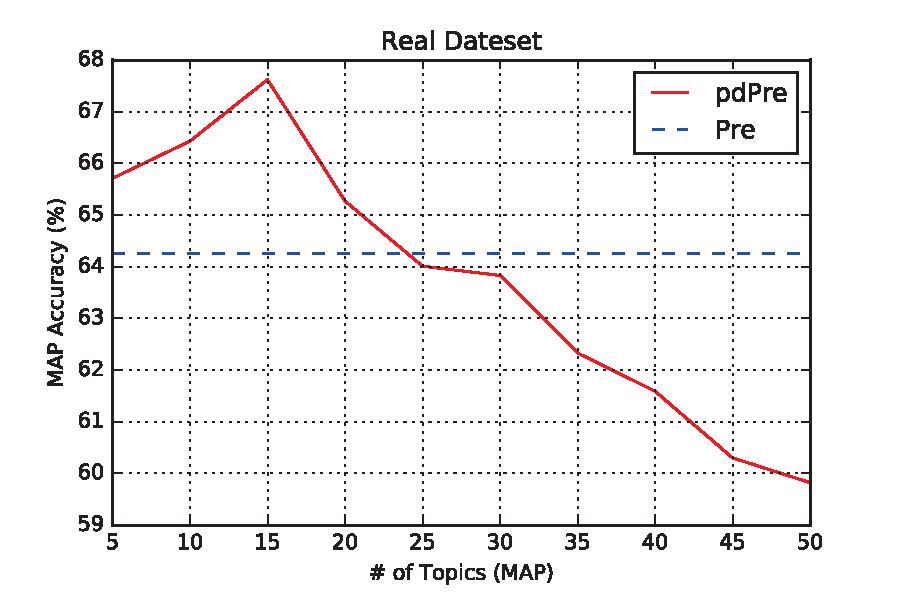
\includegraphics[width=0.49\linewidth]{05/6_rec_rank_r.pdf}}
\subfigure[虚拟账户推荐准确率]{
 \label{fig:pre_rec_a}
 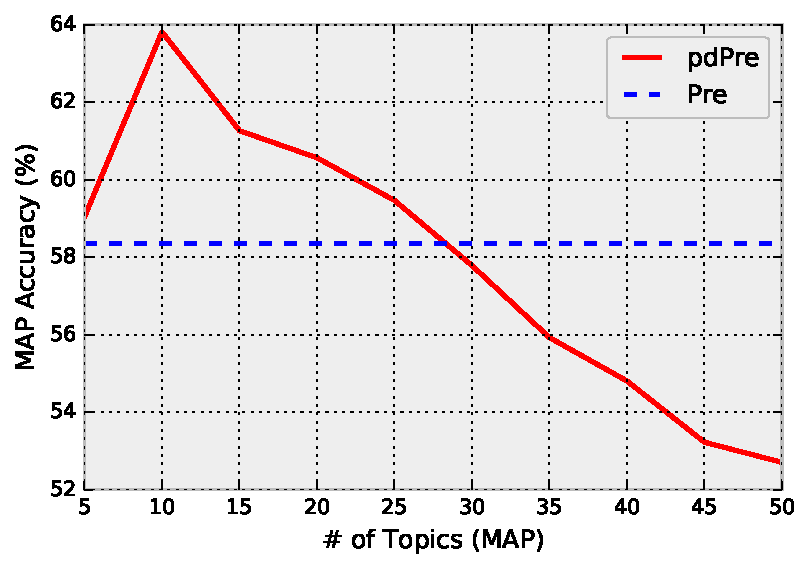
\includegraphics[width=0.49\linewidth]{05/7_rec_rank_a.pdf}}
\bicaption[fig:pred_rec]{机票推荐}{两个数据集上机票推荐准确率}{Fig}{Mean Accuracy for Flight Ticket Recommendation on Datasets}
\end{figure}

图\ref{fig:pred_rec}展示了机票推荐的实验结果。其中图\ref{fig:pre_rec_r}是在真实账户数据集的推荐结果;图\ref{fig:pre_rec_a}是在虚拟账户数据集的实验结果。
其中,横轴是主题数量。进行机票推荐的两种方法分别是结合乘客预测的推荐(pdPre)以及不使用乘客预测的推荐(Pre)。可以看到,推荐结果随着主题数量的变化有较大的波动。并且其变化趋势与乘客预测准确率较为吻合。当主体数量在10到15时,推荐准确率达到峰值;当主题数量在25到30时,推荐效果反而差于不进行乘客预测的推荐。因为此时进行乘客预测的准确率较低,而无法做出有针对性的乘客模型融合。另外,在虚拟数据集上机票推荐准确率低于真实数据集。因为由不同账户抽取出的乘客偏好会有较大差异。如果将其视作一个账户进行偏好建模,会对推荐结果产生影响。同样,虚拟数据集对推荐效果的提升程度高于真实数据集。由此我们可以得出结论:在较高的乘客预测准确率的保障下,乘客间的差异越大,
结合乘客预测的机票推荐准确率提升越大。


\begin{figure}
\centering
\subfigure[真实账户推荐Top-N准确率]{
 \label{fig:pre_top_r}
 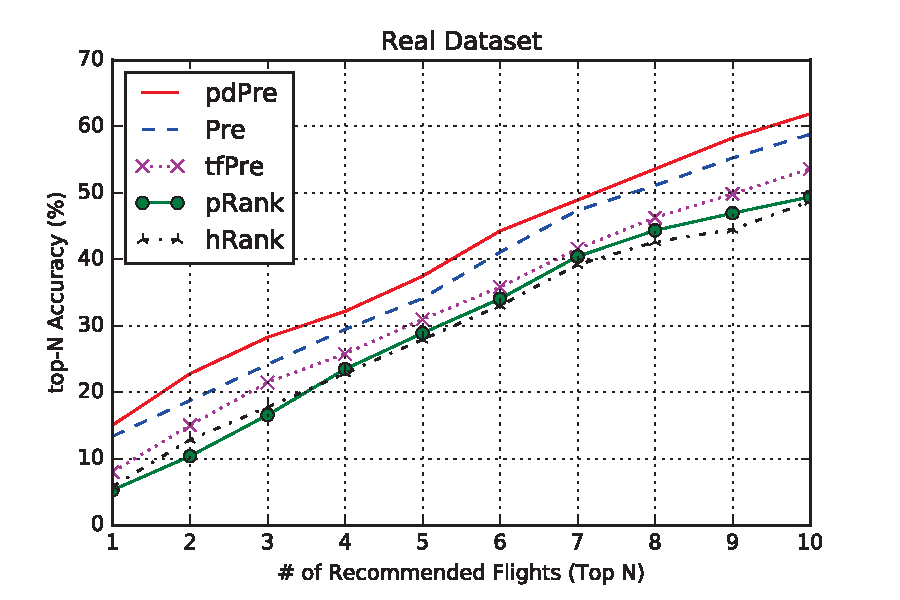
\includegraphics[width=0.49\linewidth]{05/8_rec_top_r.pdf}}
\subfigure[虚拟账户推荐Top-N准确率]{
 \label{fig:pre_top_a}
 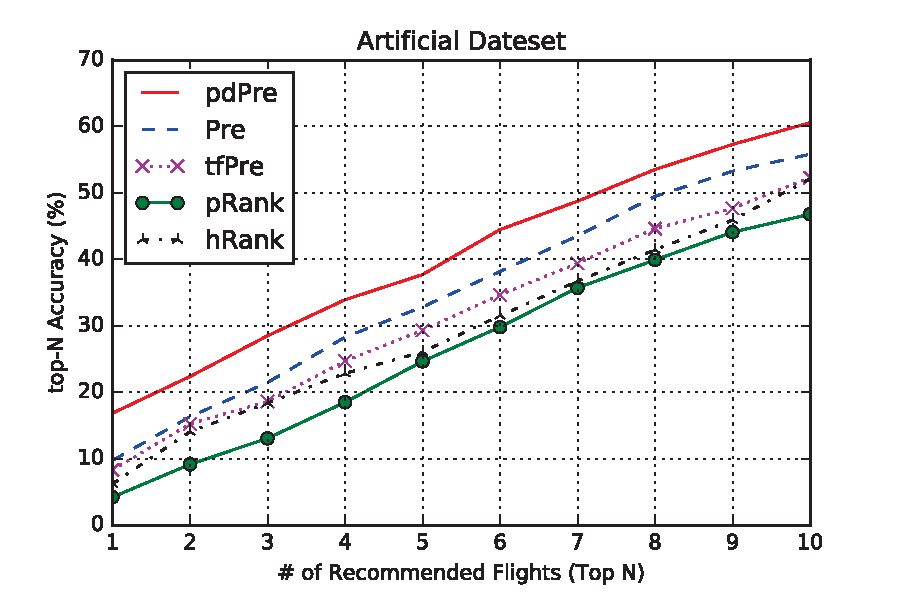
\includegraphics[width=0.49\linewidth]{05/9_rec_top_a.pdf}}
\bicaption[fig:pred_top]{机票推荐Top-N}{两个数据集上机票推荐Top-N准确率}{Fig}{Top-N Accuracy for Flight Ticket Recommendation on Datasets}
\end{figure}

图\ref{fig:pred_top}展示了机票推荐的实验结果。其中图\ref{fig:pre_top_r}是在真实账户数据集的推荐结果;图\ref{fig:pre_top_a}是在虚拟账户数据集的实验结果。在该实验中,我们将ATM模型的主题数量固定在10。
其中,横轴是$Top-N$策略中推荐机票的条数。在$Top-N$方法中,我们一并计较了基于低价排序(pRank)和热门程度(hRank)排序的推荐准确率。可以看到,几种基于策略的推荐方法的准确率与基于用户特征分布模型的推荐准确率有较大的差异。并且推荐条数从1到10,结合乘客预测的机票推荐(pdPre)都比不进行乘客预测的机票推荐(Pre)具有更高的准确率。在虚拟数据集上的推荐准确率提升高于真实数据集。


\section{本章小结}

本章我们研究了机票用户中的乘客共享账户问题。并基于可以获取账户成员真实信息的场景提出了使用作者-主题模型的乘客预测模型。首先我们预定义了机票特征及上下文词库。在模型训练过程中,我们将每个账户的所有订单作为一个语料库,每条订单作为一个文档,订单的特征取值区间作为一个单词。使用Gibbs取样进行参数推导。并就当前会话的上下文信息给出乘客预测结果。

得到乘客预测结果后,我们将乘客预测结合到机票推荐流程中。我们介绍了推荐流程的概况以及为用户更新ATM模型的过程。使得该模型具有实际应用价值。在实验章节,我们对乘客预测和结合乘客预测的机票推荐进行了数据实验并分析了实验结果。可以说明,ATM模型对乘客预测的准确率有较好的提升效果,并且结合了乘客预测的特征分布模型可以提升个性化机票推荐的准确率。